
%!TEX ROOT=ctutest.tex

\chapter{Identifikace systému}

U robotického manipulátoru zpravidla nejsou zcela známy informace o dynamických parametrech robota, jako jsou momenty setrvačnosti, hmotnosti nebo koeficienty tření jednotlivých os. Tyto informace nejsou v běžných situacích poskytovány ani samotnými výrobci robotů. Je to hlavně proto, že pro zákazníka nejsou tyto údaje důležité, protože se robotické manipulátory dodávají jako hotové uzavřené systémy připravené k použití a jejich řízení je již výrobcem implementováno v jejich řídicím systému.

\section{Způsoby identifikace}

Protože obvykle nejsou známy všechny dynamické parametry, je pro vytvoření dynamického modelu nutné tyto parametry nějakým způsobem získat nebo odvodit. Toho je možné docílit několika způsoby.

\subsection{Přímé měření součástí robota}

Dynamické parametry je možné určit rozebráním robota na menší součásti a přímým měřením jejich dynamických vlastností. Tento způsob se jeví jako nejpřirozenější.

Určení parametrů takovýmto způsobem je ale možné pouze u jednoduchých laboratorních modelů robota tvořených malým počtem součástí. U větších a složitějších robotů, jako jsou průmyslové manipulátory, je tento způsob náročný časově i způsobem provedení. Jednotlivá ramena sestávají z více komponent, jako jsou samotné kostry ramen, převodovky motorů, napájecí a komunikační vedení motorů a dalších. Ty mohou dále sestávat z dalších součástek. Rozebrání robota navíc může způsobit ztrátu podpory a záruky ze strany výrobce.

Další nevýhodou je to, že tento způsob není možné zobecnit na více typů robotů. Každý nový typ robotu by bylo nutné rozebrat a změřit, i kdyby se jednalo o robota podobného typu a konstrukce. Proto se tato práce tímto postupem dále nezabývá.    

\subsection{Použití 3D modelu}

Výrobci často poskytují ke stažení 3D modely svých robotů. Obvykle tyto modely slouží pro účely vytvoření počítačových simulací nebo modelů výrobních linek. 
3D modely je možné použít ke zjištění neznámých dynamických parametrů jejich analýzou v nástrojích CAD, jako je například AutoCAD nebo Siemens NX. Tyto nástroje jsou schopny z geometrie objektů počítat jejich objemy, momenty setrvačnosti, polohy těžišť a hmotnosti.

Výhodou tohoto postupu je jeho rychlost a jednoduchost. Navíc je takto možné získat požadované parametry i bez nutnosti přístupu k opravdovému fyzickému robotu. Tento postup je také možné zobecnit na libovolný typ robotického manipulátoru. Stačí k němu jen mít jeho odpovídající 3D model. 3D model robotu KUKA KR5 Arc v prostředí Siemens NX 10.0 je na obrázku \ref{kuka_3d_pic}.

\begin{figure}[ht]
    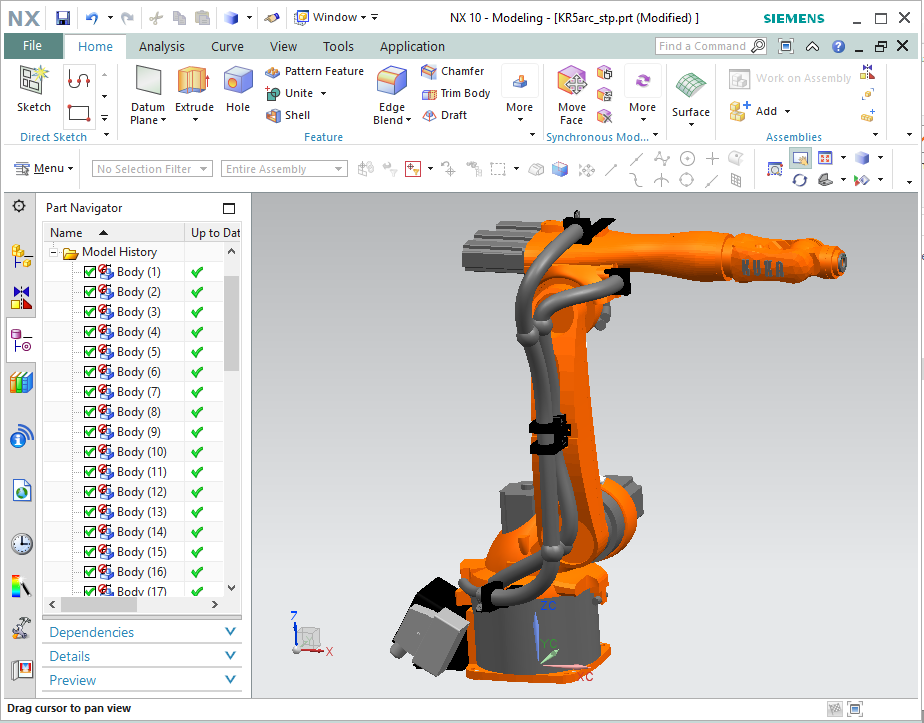
\includegraphics[width=0.8\textwidth]{kuka_3d}
    \caption{3D model robotu KUKA KR5 Arc v prostředí Siemens NX 10.0.}
    \label{kuka_3d_pic}
\end{figure}

3D model ale zpravidla popisuje pouze povrchovou geometrii jednotlivých komponent robota a neobsahuje informace o jejich vnitřní konstrukci, typech použitých materiálů, jejich skutečných hmotnostech nebo hustotách. Je zde možnost považovat jednotlivé součásti robotu za tělesa s homogenní hustotou a hmotnosti odhadnout z celkové hmotnosti robotu, která bývá udávána v jeho dokumentaci. Tento postup ale dává jen velmi hrubý odhad dynamických parametrů. 

Navíc z 3D modelu není možné získat informace o koeficientech tření v jednotlivých osách. 

Tento způsob identifikace je v této práci použit pouze pro účely porovnání určených hodnot s hodnotami odvozenými metodou popsanou v sekci \ref{z_rovnic_sec}.
\label{z_3d_modelu_sec}

\subsection{Analytické rovnice}
\label{z_rovnic_sec}
Neznámé dynamické parametry je možné přesně vypočítat pomocí dynamických rovnic robota. 

Přestože jsou dynamické rovnice robotu \eqref{celkova_dyn_rovnice_eq} nelineární vůči jednotlivým zobecněným souřadnicím (polohy, úhlové rychlosti a úhlová zrychlení na jednotlivých osách), jsou lineární vůči jednotlivým složkám dynamických parametrů \cite{clos_dyn_par}\cite{dyn_mod_ind}. Proto je tyto rovnice možné přepsat do tvaru

\begin{equation}
\vect{T_r} = \mathbb{H}(\vect{\ddot{\theta}},\vect{\dot{\theta}},\vect{\theta})\vect{R},
\label{eq_lin_par}
\end{equation}
kde
\begin{description}
\item[$\vect{T_r} = {\big[T_{r1}, T_{r2},  \dotsm  T_{rn}\big]}^{T}$] je vektor momentů sil na osách v čase $t$ ,
\item[$\vect{R} = {\big[\vect{R_1}, \vect{R_2},  \dotsm  \vect{R_n}\big]}^{T}$] je vektor neznámých dyn. parametrů jednotlivých os,
\item[$n$] je počet os
\end{description} \noindent
a \ \ \ \ \ \ $\vect{R_i} = {\big[I_{ixx}, \ I_{ixy}, \ I_{iyy}, \ I_{iyz}, \ I_{izz}, \ I_{izx}, \ m_i, \ m_id_{ix}, \ m_id_{iy}, \ m_id_{iz}, \ f_{vi}, \ f_{ci}\big]}$, \\
\\
\\
kde
\noindent
\begin{description}
\item[$I_{ijk}$] je složka setrvačnosti pro link $i$ vůči kartézským souřadnicím $j$ a $k$,
\item[$r_{ij}$] je složka vektoru těžiště linku $i$ vyjádřená v kartézské souřadnici $j$,
\item[$m_{i}$] je hmotnost linku $i$,
\item[$f_{vi}$] je koeficient viskózního tření linku $i$,
\item[$f_{ci}$] je koeficient Coulombova tření linku $i$.
\end{description}

Počet neznámých parametrů pro jedno rameno robotu odpovídá počtu složek vektoru $\vect{R_i}$. Ten je roven 12. U sériového průmyslového manipulátoru se šesti rotačními osami je tedy neznámých parametrů celkem 72. 

Počet neznámých parametrů je možné zredukovat. Je to možné díky tomu, že některé parametry dynamiku robota neovlivní nebo je jejich vliv zanedbatelný. Důvodem je to, že se některé linky mohou otáčet pouze kolem některé z os. Příkladem může být osa 1 (spojená se zemí, viz schéma \ref{kuka_kr5_axes_pic}), která se v prostoru může otáčet jen kolem vertikální osy. Tím je možné zanedbat momenty setrvačnosti mimo tuto vertikální osu. Zároveň je možné model dále zjednodušit uvažováním pouze prvků na hlavní diagonále tenzorů setrvačnosti a zanedbáním prvků mimo ni. Touto aproximací je snížena přesnost modelu, ale zároveň se tím významně zjednoduší model. Dále jsou některé dynamické parametry robotu jsou sdruženy. Příkladem může být moment setrvačnosti a poloha těžiště osy 1 nebo polohy těžišť os 3 a 4.

Díky tomu klesne počet neznámých parametrů v případě šestiosového robotu z čísla 72 na číslo 48. V tabulce \ref{tab_hled_param} je přehled výsledných neznámých dynamických parametrů robota KUKA KR5 Arc.
\\

\begin{table}[ht]
  \centering
  \caption{Tabulka nezámých parametrů robota KUKA KR5 Arc.}
    \begin{tabular}{c|lllllllll}
    \multicolumn{1}{c|}{Osa} & \multicolumn{9}{c}{Neznámé parametry}  \\
    \hline
    1 &       	  &	          & $I_{1zz}$ &          &          &          & & $f_{v1}$ & $f_{c1}$ \\
    2 & $I_{2xx}$ & $I_{2yy}$ & $I_{2zz}$ & $d_{2x}$ & $d_{2y}$ & $d_{2z}$ & $m_{2}$ & $f_{v2}$ & $f_{c2}$ \\
    3 & $I_{3xx}$ & $I_{3yy}$ & $I_{3zz}$ & $d_{3x}$ & $d_{3y}$ & $d_{3z}$ & $m_{3}$ & $f_{v3}$ & $f_{c3}$ \\
    4 & $I_{4xx}$ & $I_{4yy}$ & $I_{4zz}$ & $d_{4x}$ & $d_{4y}$ & $d_{4z}$ & $m_{4}$ & $f_{v4}$ & $f_{c4}$ \\
    5 & $I_{5xx}$ & $I_{5yy}$ & $I_{5zz}$ & $d_{5x}$ & $d_{5y}$ & $d_{5z}$ & $m_{5}$ & $f_{v5}$ & $f_{c5}$ \\
    6 & $I_{6xx}$ & $I_{6yy}$ & $I_{6zz}$ & $d_{6x}$ & $d_{6y}$ & $d_{6z}$ & $m_{6}$ & $f_{v6}$ & $f_{c6}$ \\
    \end{tabular}%
  \label{tab_hled_param}%
\end{table}%

Hledané parametry je poté možné vypočítat z rovnice \eqref{eq_lin_par} jejich vyjádřením ve tvaru

\begin{equation}
\vect{R} = \mathbb{H}\big(\vect{\ddot{\theta}},\vect{\dot{\theta}},\vect{\theta}\big)^{-1}\vect{T}.
\label{eq_lin_par_inv}
\end{equation}

K výpočtu vektoru $\vect{R}$ neznámých parametrů je potřeba s robotem vykonat pohyb po identifikační trajektorii a měřit polohy, úhlové rychlostí, úhlová zrychlení a momenty sil na jednotlivých osách. Do matice $\mathbb{H}\big(\vect{\ddot{\theta}},\vect{\dot{\theta}},\vect{\theta})$ jsou poté dosazeny tyto změřené polohy, úhlové rychlosti a úhlová zrychlení jednotlivých os v čase $t$ a do vektoru $\vect{T}$ změřené momenty sil v čase $t$. 

Protože je ale neznámých parametrů více než rovnic, nelze tuto rovnici vyřešit jednoznačně. Tento problém lze jednoduše vyřešit naměřením více bodů na trajektorii v různých časech a jejich následným dosazením do rovnice \eqref{eq_lin_par_inv}. Důležité je na trajektorii mít změřen takový počet bodů, aby z této rovnice vznikla rovnice přeurčená. Takovou přeurčenou rovnici je poté možné řešit například použitím metody nejmenších čtverců, která minimalizuje střední odchylku mezi skutečnými a odhadnutými parametry a navíc je schopna potlačit vliv šumu měření. 

\subsection{Excitační trajektorie}

Neznámé parametry identifikované postupem popsaným v sekci \ref{eq_lin_par} jsou silně závislé na zvolené trajektorii, na které jsou měřeny průběhy dynamických veličin. 

Aby tímto způsobem bylo možné správně odhadnout hodnoty všech neznámých parametrů, je potřeba s robotem vykonat pohyby po takové trajektorii, na které jsou vybuzeny všechny dynamické složky robota. Trajektorie musí být zvolena tak, aby se do dynamiky pohybu promítly všechny neznámé parametry. Identifikace z nedostatečně budící (excitující) trajektorie sice také odhadne všechny neznámé parametry, model s nimi ale bude přesný pouze pro pohyby po této trajektorii nebo v jejím okolí.

Ve vědeckých článcích a publikacích např. \cite{dyn_mod_ind}\cite{dyn_ind_mits}\cite{clos_dyn_par} se na jednotlivých osách jako excitační trajektorie doporučují trajektorie, které je možné popsat konečnou Fourierovou řadou. Jejich výhodou je, že díky vlastnostem harmonických funkcí jsou poté jednotlivé polohy, rychlosti i zrychlení rovněž lineární kombinací harmonických průběhů. Tím je maximalizován vliv hledaných dynamických parametrů a minimalizován vliv šumu měření. 

Protože se průmyslové manipulátory používají převážně pro polohování, je obtížné vykonávat na osách čistě harmonické průběhy. Řídicí systém robota KUKA KR5 Arc umožňuje zadat požadovanou trajektorii dvěma hlavními způsoby. První způsob je zadání trajektorie jako sady požadovaných poloh os, kterých musí osy dosáhnout a rychlosti/zrychlení, s jakými se má tento pohyb vykonat. Druhou možností je zadání požadovaných poloh a rychlostí koncového efektoru v kartézských souřadnicích. Řídicí systém následně sám přechod mezi těmito zadanými polohami aproximuje hladkou trajektorií. 

Z tohoto důvodu je nutné robotu poskytnout sérii bodů popisujících harmonický průběh. Výsledná trajektorie robota je poté pouze aproximací harmonického průběhu.  

\section{Postup identifikace}

Identifikaci parametrů robota KUKA KR5 Arc byla provedena způsobem popsaným výše v sekci \ref{z_rovnic_sec}. 

Pomocí nástroje ReDySim byla vygenerována soustava šesti rovnic dynamiky robota. Protože ReDySim v rovnicích neuvažuje tření na jednotlivých osách, bylo nutné toto tření do vygenerovaných rovnic ručně doplnit. Výsledná soustava rovnic poté byla převedena do maticového tvaru lineárního vůči neznámým dynamickým parametrům (rovnice \eqref{eq_lin_par}). 

\newpage
Za vektor $\vect{R}$ neznámých parametrů byl zvolen vektor s parametry všech šesti os

$\vect{R} = [\begin{matrix} \vect{R_i}, & \vect{R_{md}}, & \vect{R_f} \end{matrix}]^{T},$

kde 
\begin{description}
\item[$  \vect{R_i} = {\big[I_{1x}, \ I_{1y}, \ I_{1z}, \ \cdots \ , I_{6x}, \ I_{6y}, \ I_{6z}\big]}$], 
\item[$\vect{R_{md}} = {\big[m_1, \ m_1d_{1x}, \ m_1d_{1y}, \ m_1d_{1z}, \ \cdots \ , m_6, \ m_6d_{6x}, \ m_6d_{6y}, \ m_6d_{6z}\big]}$], 
\item[$\vect{R_f} = {\big[f_{v1}, \ f_{c1}, \ \cdots \ ,f_{v6} \ , f_{c6}\big]}.$] 
\end{description}

%\[\addtolength{\arraycolsep}{-1.5pt}
%\begin{split}
%R &= 
%[\begin{matrix} I_{1x} & I_{1y} & I_{1z} &\cdots &I_{6x} & I_{6y} & I_{6z} %\end{matrix} \\
% &\qquad\qquad \begin{matrix}  m_1 & m_1d_{1x} & m_1d_{1y} & m_1d_{1z} &\cdots & m_6 & m_6d_{6x} & m_6d_{6y} & m_6d_{6z} \end{matrix} \\
% &\qquad\qquad\qquad\qquad \begin{matrix} f_{v1} & f_{c1} &\cdots & f_{v6} & f_{c6} \end{matrix}]^{T}
%\end{split}
%\]

Do matic $\mathbb{H}\big(\vect{\ddot{\theta}},\vect{\dot{\theta}},\vect{\theta}\big)$ a $\vect{T}$ byly dosazeny jednotlivé polohy os, úhlové rychlosti, úhlová zrychlení a momenty sil naměřené v různých časech na identifikační trajektorii. Vektor neznámých parametrů $R$ byl poté vypočítán z rovnice \eqref{eq_lin_par_inv} metodou nejmenších čtverců podle vztahu

\begin{equation}
\begin{split}
\arg\min_{R} \frac{1}{2}\lvert|\mathbb{H}\vect{R}-\vect{T}\rvert|_2^2, \\
\vect{lb} < \vect{R} < \vect{ub},
\end{split}
\label{lsq}
\end{equation}

kde $\vect{lb}$ je vektor dolních hranic hledaných hodnot a $\vect{ub}$ je vektor jejich horních hranic.

Protože jsou dynamické rovnice robota silně nelineární, může se stát, že solver metody nejmenších čtverců nenalezne globálně optimální řešení, ale skončí v některém z lokálních minim. Je také možné, že solver nalezne řešení, které bude správně matematicky, fyzikálně ale nebude dávat smysl (záporné hmotnosti ramen, apod.). Z tohoto důvodu je vhodné nějakým způsobem omezit prostor, ve kterém se má řešení hledat.

V této práci byl pro řešení metody nejmenších čtverců v MATLABu použit solver \texttt{lsqlin}, který umožňuje specifikovat hranice, ve kterých má být hledáno řešení. První z omezujících podmínek bylo, že všechny hmotnosti a momenty setrvačnosti mají mít kladné hodnoty. Dále bylo nastaveno omezení na hledané polohy těžišť ramen tak, aby tato těžiště neležela mimo fyzický objem ramen. Posledním z požadovaných omezení bylo nastavení přesných hmotností ramen, které bylo možné dohledat ve zdrojových datech robotu.

\label{postup_identifikace_ch}

\subsection{Identifikační trajektorie}

Protože je prostor kolem robotu omezen, není možné s robotem provádět pohyby v jeho plném rozsahu. Proto tomu bylo nutné přizpůsobit identifikační trajektorii. Identifikační trajektorie byla vytvořena složením několika nezávislých trajektorií. Na celkovou dynamiku robotu mají výraznější vliv osy 1-3 než osy 4-6. Proto je výhodné tyto osy identifikovat separátně. 

V první části trajektorie byl proveden pohyb pouze s posledními třemi osami (osa 6, osa 5 a osa 4). Ostatní osy byly v pevně zafixované pozici. Nejprve byl vykonán opakovaný pohyb pouze poslední šestou osou v jejím maximálním možném rozsahu v obou směrech otáčení. K tomu byl následně přidán obdobný pohyb páté osy a nakonec byl stejným způsobem přidán i pohyb čtvrté osy. Tímto byla pokryta maximální možná škála pohybů posledních tří os.

Následovala část trajektorie pro identifikaci parametrů prvních tří os. U těchto os je situace zkomplikovaná tím, že osa 2 a osa 3 mají vždy vzájemně rovnoběžné osy otáčení (viz obrázek \ref{kuka_kr5_axes_pic}). Proto je obtížné nezávisle identifikovat některé z jejich parametrů. 

V tomto případě byl postup takový, že nejprve byl vykonán opakovaný pohyb osy 3 v jejím plném rozsahu a byly zafixovány os 1 a 2. Následně byla zafixována osa 3 a stejným způsobem bylo pohybováno osou 2. Tímto byly pokryty pohyby nezávislé na rotaci kolem osy 1. 

Trajektorie závislá na pohybu osy 1 byla vytvořena tak, že nejprve byl několikrát proveden pohyb osou 1 s rameny os 2 a 3 pevně zafixovanými ve vertikální poloze. Poté byly stejné pohyby provedeny s ramenem osy 3 v horizontální poloze a následně s oběma rameny 2 a 3 v horizontální poloze.

Výsledná identifikační trajektorie byla vytvořena spojením těchto tří trajektorií v jednu. Nástroj TRACE přitom byl nastaven tak, aby prováděl měření poloh, úhlových rychlostí, úhlových zrychlení, momentů sil a proudů na všech osách. 

\section{Identifikační skript pro MATLAB}

Pro účely identifikace robota KUKA KR5 Arc byl vytvořen skript pro použití v MATLABu, který umožňuje vytvoření dynamického modelu, načtení změřených trajektorií, identifikaci neznámých parametrů, simulaci a srovnání výsledků a analýzu vlivu nepřesnosti odhadnutých parametrů na přesnost modelu.

Skript je rozdělen na několik po sobě jdoucích podprogramů, které je možné spouštět vcelku nebo po jednotlivých částech. Komentáře ve skriptu jsou psány v anglickém jazyce pro případné rozšíření jeho použití. Diagram znázorňující jednotlivé podprogramy ve skriptu je na obrázku \ref{diagram_pic}.

První část je univerzální pro libovolného sériového robota s rotačními osami. Definují se zde základní parametry robotu, jako je počet os, délky jednotlivých ramen, převodní poměry převodovek a počet měřených veličin. Dále se zde zadávají parametry motorů, mezi něž patří momentové konstanty a odpory a indukčnosti vinutí. 

\begin{figure}[ht]
    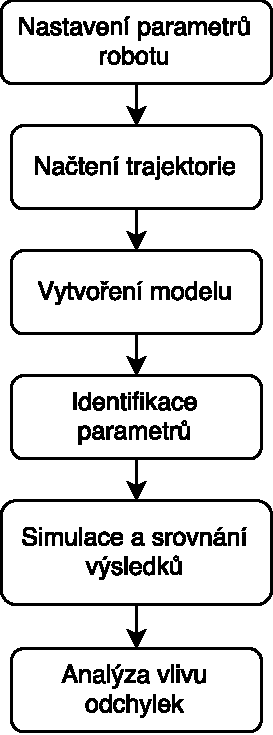
\includegraphics[width=0.25\textwidth]{diagram}
    \caption{Diagram funkce identifikačního skriptu}
    \label{diagram_pic}
\end{figure}

Další část je částečně závislá na použitém robotu. V této části je importována změřená trajektorie robota. Robot KUKA KR5 Arc používá k měření trajektorií nástroj TRACE. Tento nástroj ukládá změřená data ve speciální struktuře ve formátu .r64. Tu je potřeba rozložit na jednotlivé měřené složky a ty dále vynásobit převodními koeficienty měření. Jiné typy robotů, obzvláště roboty od jiných výrobců budou pravděpodobně mít změřené trajektorie ukládány jiným způsobem a v jiných formátech. Proto je potřeba, v případě použití jiného robotu, skript upravit nebo doplnit pro správné importování těchto dat. Výsledkem této části je trojrozměrná matice naměřených trajektorií pro jednotlivé osy a veličiny. 

Následující části jsou již zcela nezávislé na robotické platformě a jsou univerzální pro použití pro libovolného robota.  

Nejprve je vytvořen vektor $\vect{R}$ parametrů v symbolickém tvaru. Následuje načtení vygenerovaných rovnic z nástroje ReDySim, jejich převod do symbolického tvaru a uložení do matice rovnic. Z té je poté vygenerovaná matice $\mathbb{H}_i\big(\vect{\ddot{\theta}},\vect{\dot{\theta}},\vect{\theta}\big)$ se symbolickými proměnnými, do kterých je možné dosazovat změřená data.

Postupným dosazováním naměřených bodů na trajektorii (polohy, úhlové rychlosti a úhlová zrychlení) do matice $\mathbb{H}_i\big(\vect{\ddot{\theta}},\vect{\dot{\theta}},\vect{\theta}\big)$ je vytvořena matice $\mathbb{H}$. Současně je vytvořen vektor $\vect{T}$ s dosazenými změřenými momenty sil.

\newpage
Tyto vektory a matice jsou poté předány solveru \texttt{lsqlin}, který vypočte vektor $\vect{R}$ vyřešením rovnice \eqref{eq_lin_par_inv} metodou nejmenších čtverců. Zároveň je zde možné nastavit horní i spodní hranice jednotlivých parametrů vektoru $\vect{R}$ ve kterých má solver řešení hledat.

Model s odvozenými parametry je možné v další části hned odsimulovat a porovnat se skutečnými změřenými trajektoriemi.

V poslední části je provedena analýza vlivu odchylek v hodnotách parametrů na přesnost energetického modelu robotu. Analýza vlivu odchylek je provedena pomocí metody Monte Carlo. Model je v cyklu odsimulován 200 krát pokaždé s jinou náhodně vygenerovanou hodnotou přičtenou k parametru. Poté je vypočítána střední odchylka mezi simulací a měřením. Tento postup je v cyklu opakován pro všechny identifikované parametry. 

Následuje vyhodnocení těchto výsledku a nalezení případů, kdy byla odchylka mezi modelem a změřenými hodnotami největší. Ve skriptu je možné upravovat počet simulací a rozsah odchylek parametrů.  

